% !TEX root = paper.tex

\documentclass[11pt,letterpaper]{article}

% Packages
\usepackage{packages}
\addbibresource{sources.bib}

% Document Settings
\geometry{margin=1in}
\setlength{\parskip}{1ex}
\setlength{\parindent}{0pt}

% =========================================
%             DOCUMENT
% =========================================

\begin{document}
\doublespacing % Double spacing throughout the document


% =========================
%      TITLE PAGE
% =========================

% Suppresses headers, footers, and page numbers on title page
\begin{titlepage}
    \begin{center}
    \vspace*{4cm}
    A statistical approach to predicting a tsunami’s wave height \\
    \vspace{1cm}
    Can the height of a tsunami's wave be predicted based on the distance from and 
    the magnitude of a preceding earthquake? \\
    \vspace{4cm}
    Word count: TBD
    \vfill
    \vspace{0.1cm}
    \end{center}
    \end{titlepage}

% =========================
%      DOCUMENT BODY
% =========================

\pagenumbering{roman}

\begin{center}
\pdfbookmark{\contentsname}{Contents}
\tableofcontents
\vspace{1in}

\end{center}


% TODO: Add hyper-references to links
% TODO: Improve listings' styling
% TODO: Add links to Contents entries

\newpage

\pagenumbering{arabic}

\section{Introduction}

\subsection{Background}

Naturally occurring disasters such as tsunamis are devastating for 
people and resources residing in risk areas. These tsunamis are caused 
by many different types of natural phenomena such as landslides, collapse of 
seamount, or more rarely, the impact of a meteorite. This paper however will focus 
on one of the more common cases of tsunami; one caused by the earthquakes. This 
is due to earthquakes causing around 72\% of earthquakes \cite{pacifictsunamimuseum}, and as the time between an 
earthquake event and its tsunami is relatively high compared to events such as landslides \cite{sue_nokes_walters}, 
leaving adequate time for prediction and correct preparation of the events properties, such as 
the wave height, as discussed in this paper. 

\subsection{Personal Engagement}

I have chosen to write about this subject as I have recently become interested by the 
statistics and its implications in real-life matters. This research has proved very 
interesting for me as it has abstracted the field of statistics for me. Furthermore, 
as I enjoy programming, the research I have done has helped me learn about the tools 
and technologies used by data analysts and other professionals of the matter. 


\section{}


\section{Statistical Model}

\subsection{Processing the dataset for use}

The dataset, procured from the NOAA website \cite{noaa}, includes many tsunami 
runups, going back before the year 0. Due to this, the NOAA states uncertainties 
that can occur in its data. For example, reports that were recorded before the 
20th century tend to be based on written accounts, and not recorded seismic activity. 
Furthermore, the installation of a system called the Worldwide Standardized Seismograph 
Network in the 1960s allowed for more accurate data and for that reason any recorded 
activity before this date will be discarded from the dataset. The dataset itself can 
be accessed through two different methods; searching the database using the online 
tool or downloading it in a somewhat obscure Google Earth format. The online tool 
supports the download of search results in a much more human-readable \verb|.csv| format, 
so I search for all entries after the year 1900, and downloaded the result. 

The data is cleaned of all "dubious" reports, reports before the year 1960 (see above), and 
of all irrelevant fields such as "Injuries" or "Damage \$Mil". This preliminary data cleanup 
is done through the use of the pandas Python library \cite{reback2020pandas}\cite{mckinney-proc-scipy-2010}, 

The data must be then correctly split into a training and an test dataset. The training 
dataset will be used to generate a regression model while the test dataset will 
be used to calculate the general accuracy of the model, by predicting values and 
comparing those to the known value as found in the dataset. The dataset is split based on 
a decimal number using the \verb|df.sample| method found in the pandas library. A split 
of 70\% for training and 30\% for test has been chosen. A \verb|random_state| argument is 
set to an arbitrary value 42, as if it weren't, the dataset would be split in a different 
manner at each execution of the program. 

\subsection{Regression}

Regression analysis is a very large portion of statistics, and regression models can 
be found in numerous use cases of the field. Regression models consist of estimating the 
relationship between one (or more) independent variables and a dependent variable. A 
simple example of regression can be seen in the linear relationship between an independent 
variable $x_{i}$, and the dependent variable $y$. The following expression shows this relationship in what is 
called linear regression, as it models a straight line. 

$y = a + \beta x + e $

Where the term $a$ represents the y-intercept of the line and $\beta$ represents the 
coefficient of $x_i$. The final term $e$ is what is known as the error or residual 
term, it is an estimate of the amount by which the predictions differ from the real 
value. 

However, the relationship between the distance from an event and the wave height 
is not necessarily linear, especially if it is considered that the travel of 
sound in a fluid obeys the inverse square law. This already tells us a simple 
linear regression model cannot be used for this research. If we want a second degree 
polynomial regression formula, a new $x^2$ term can be added to the previous formula 
and we get: 

$y = a + \beta_1 x + \beta_2 x^2 + e$

Even though the right side of this equation is quadratic in $x$, this is still 
linear regression as the right side is linear in $\beta$ (if we were to let 
$x = 1$, we would be left with $y = a + \beta_1 + \beta_2 + e$, which is linear). 
A second degree polynomial regression would best fit our model for both independent 
variables, as seen in the graphs below, where a theoretical regression line is drawn 
by hand:

\begin{figure}[h]
    \centering
    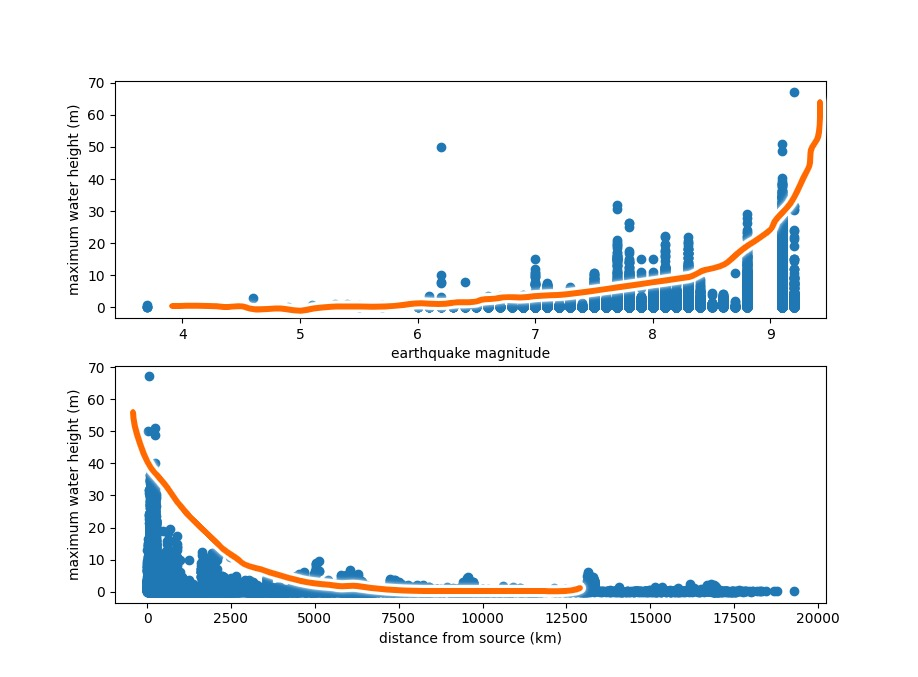
\includegraphics[width=0.8\textwidth]{modelshowcase.jpeg}
    \label{fig:boat1}
\end{figure}

In addition, our dataset has two independent variables: the distance from a particular 
earthquake event and the magnitude of that earthquake. 





\dots

So the relationship between the two independent variables and the wave height can 
be estimated with a multivariate, polynomial regression model. We will use the Python 
scikit-learn library to aid in creating this model.  


\dots

The model's accuracy is then calculated, with the mentioned before "test" dataset. 
The \verb|accuracy_score| method from the \verb|sklearn.metrics| class is used for this 
task. 

\dots



\subsection{Ease of access}
For an easy access to the predictions generated by the program, I implemented 
a simple function to fetch new earthquake events from the \url{https://earthquake.usgs.gov/earthquakes/feed/v1.0/geojson.php} 
live earthquake feed. These earthquake events are quantified into a magnitude \verb|mag| 
and a distance \verb|dist| variable, which are supplied to the statistical model. 
This information is then easily accessible from a human-readable report exported 
to a plaintext file. Following is an example report generated by the tool: 

\section{Uses of this research}

The research included in this paper could be useful for many life-saving scenarios, 
notably ones in which, for example, high quality and large-scale tsunami alert 
systems are not available. 

\section{Conclusion}

\subsection{Evaluation of the method used}

This method, like any other statistical approximation, is by no means perfect 
and for that reason should not be used in any real-world application. The results 
procured by the program are subject to many uncertainties, one of which is described 
below.

When attempting to predict the maximum wave height of a tsunami such as the one 
caused by the 2011 earthquake off the Pacific coast of Tōhoku, approximately 70km 
away from shore, which produced a 38.9m wave \cite{yomiuri_2011}. The model in this 
paper approximates this same event as only a 8m wave, when supplied the 9.0 magnitude 
of the earthquake and the 70km distance. These types of errors can be attributed to the 
fact that there are many more independent variables, such as the shape of the seafloor for 
example, that can amplify or potentially change the height of a tsunami's wave. 
%todo add 

\printbibliography[heading=bibintoc, title=Works Cited]

\appendix
\section{Appendix}
\label{app}
\subsection{Python program}
\label{app:scripts}
qsd
\lstinputlisting[language=Python]{model/multregr.py}


\end{document}